%%%%%%%%%%%%%%%%%%%%%%%%%%%%%%%%%%%%%%%%%
% Journal Article
% LaTeX Template
% Version 1.4 (15/5/16)
%
% This template has been downloaded from:
% http://www.LaTeXTemplates.com
%
% Original author:
% Frits Wenneker (http://www.howtotex.com) with extensive modifications by
% Vel (vel@LaTeXTemplates.com)
%
% License:
% CC BY-NC-SA 3.0 (http://creativecommons.org/licenses/by-nc-sa/3.0/)
%
%%%%%%%%%%%%%%%%%%%%%%%%%%%%%%%%%%%%%%%%%

%----------------------------------------------------------------------------------------
%	PACKAGES AND OTHER DOCUMENT CONFIGURATIONS
%----------------------------------------------------------------------------------------

\documentclass[twoside,twocolumn]{article}

\usepackage{blindtext} % Package to generate dummy text throughout this template 

\usepackage[sc]{mathpazo} % Use the Palatino font
\usepackage[T1]{fontenc} % Use 8-bit encoding that has 256 glyphs
\linespread{1.05} % Line spacing - Palatino needs more space between lines
\usepackage{microtype} % Slightly tweak font spacing for aesthetics

\usepackage[french]{babel} % Language hyphenation and typographical rules
\usepackage[utf8]{inputenc}

\usepackage{graphicx}

\usepackage[hmarginratio=1:1,top=32mm,columnsep=20pt]{geometry} % Document margins
\usepackage[hang, small,labelfont=bf,up,textfont=it,up]{caption} % Custom captions under/above floats in tables or figures
\usepackage[format=plain,indention=0mm]{caption} % To change caption style
\usepackage{booktabs} % Horizontal rules in tables

\usepackage{lettrine} % The lettrine is the first enlarged letter at the beginning of the text

\usepackage{enumitem} % Customized lists
\setlist[itemize]{noitemsep} % Make itemize lists more compact

\usepackage{abstract} % Allows abstract customization
\renewcommand{\abstractnamefont}{\normalfont\bfseries} % Set the "Abstract" text to bold
\renewcommand{\abstracttextfont}{\normalfont\small\itshape} % Set the abstract itself to small italic text

\usepackage{titlesec} % Allows customization of titles
\renewcommand\thesection{\Roman{section}} % Roman numerals for the sections
\renewcommand\thesubsection{\roman{subsection}} % roman numerals for subsections
\titleformat{\section}[block]{\large\scshape\centering}{\thesection.}{1em}{} % Change the look of the section titles
\titleformat{\subsection}[block]{\large}{\thesubsection.}{1em}{} % Change the look of the section titles

\usepackage{fancyhdr} % Headers and footers
\pagestyle{fancy} % All pages have headers and footers
\fancyhead{} % Blank out the default header
\fancyfoot{} % Blank out the default footer
\fancyhead[C]{Comparaison de différentes méthodes de saisie} % Custom header text
\fancyfoot[RO,LE]{\thepage} % Custom footer text

\usepackage{titling} % Customizing the title section

\usepackage{hyperref} % For hyperlinks in the PDF




%----------------------------------------------------------------------------------------
%	TITLE SECTION
%----------------------------------------------------------------------------------------

\setlength{\droptitle}{-4\baselineskip} % Move the title up

\pretitle{\begin{center}\Huge\bfseries} % Article title formatting
\posttitle{\end{center}} % Article title closing formatting
\title{Comparaison de la méthode de saisie dichotomique sur le dictionnaire avec les méthodes d'épellation traditionnelles} % Article title
\author{%
\textsc{Équipe Dicotomix}
\normalsize ENS de Lyon \\ % Your institution
\normalsize \href{mailto:dicotomix@ens-lyon.fr}{dicotomix@ens-lyon.fr} % Your email address
%\and % Uncomment if 2 authors are required, duplicate these 4 lines if more
%\textsc{Jane Smith}\thanks{Corresponding author} \\[1ex] % Second author's name
%\normalsize University of Utah \\ % Second author's institution
%\normalsize \href{mailto:jane@smith.com}{jane@smith.com} % Second author's email address
}
\date{} % Leave empty to omit a date
\renewcommand{\maketitlehookd}{%
\begin{abstract}
%\noindent 
Les méthodes traditionnelles permettant de communiquer en se limitant à une entrée de la forme \textit{oui} ou \textit{non} sont basées sur une épellation lettre par lettre. Ici, une approche différente est considérée, où les mots sont épelés un à un par dichotomie sur l'ensemble du dictionnaire français. Cette méthode est ici comparée aux méthodes traditionnelles en vigueur dans le milieu médical. Nous montrons ainsi qu'une recherche dichotomique sur le dictionnaire permet d'écrire plus efficacement, en comparant les résultats obtenus en terme de temps de frappe de ces différentes méthodes. 
\end{abstract}
}

%----------------------------------------------------------------------------------------

\begin{document}

% Print the title
\maketitle

%----------------------------------------------------------------------------------------
%	ARTICLE CONTENTS
%----------------------------------------------------------------------------------------

\section{Introduction}

\lettrine[nindent=0em,lines=3]{L}es méthodes de saisie traditionnelles utilisées dans le milieu médical reposent toutes sur le même principe. Elles consistent à épeler les mots lettre à lettre, en parcourant l'alphabet pour chacune des lettres. Ce type de méthode peut s'avérer frustrant pour l'utilisateur, qui décide parfois même de renoncer à la communication, tant elle peut être fastidieuse. Une autre approche propose d'utiliser plus efficacement une entrée binaire afin d'écrire non pas une lettre à la fois, mais un mot à la fois. Ainsi, nous mettons ici en avant l'intérêt d'une telle méthode, en les comparant sur l'ensemble du dictionnaire.

%------------------------------------------------

\section{Méthodes traditionnelles}

Toutes les méthodes traditionnelles reposent sur une division de l'alphabet en une table en deux dimensions, où la recherche de la lettre voulue se fait en deux temps. Dans un premier temps, on recherche la ligne dans laquelle se situe la lettre voulue, en posant la question ``est-ce que ma lettre est dans la \textit{première} ligne'', ou dans la \textit{seconde}, jusqu'à arriver à la bonne ligne. Ensuite, on itère de la même manière sur chacune des lettres de la ligne jusqu'à trouver la lettre voulue.

Une des méthodes d'épellation les plus répandues utilise l'alphabet EJASINT décrit dans la figure \ref{ejasint}. Les autres méthodes envisagées ici sont décrites en annexe, et reposent toutes sur ce même principe de grille de lettres, avec une répartition différente de l'alphabet.
\begin{center}
\begin{figure}
  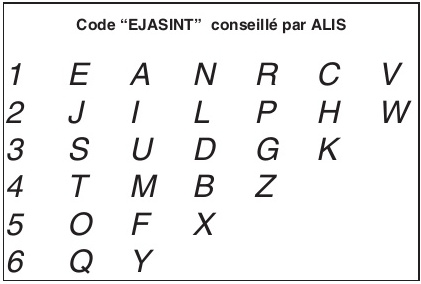
\includegraphics[scale=0.45]{ejasint.jpg}
  \caption{Alphabet EJASINT, majoritairement utilisé pour la saisie lettre à lettre par l'association ALIS}
  \label{ejasint}
\end{figure}
\end{center}

%------------------------------------------------

\section{Méthode dichotomique}

Notre méthode repose sur un parcours du dictionnaire français par dichotomie, en tenant compte des fréquences des mots dans l'usage courant de la langue française. La question posée porte ainsi sur des mots et n'est plus de la forme ``est-ce le bon mot ?'', mais ``est-il avant ou après dans l'alphabet ?''

Une seconde méthode que nous évoquerons est la méthode de l'épellation dichotomique, reprenant le principe de la dichotomie mais cette fois pour une épellation lettre par lettre : ``la lettre recherchée est-elle avant ou après dans l'alphabet ?''.

L'intérêt de l'approche dichotomique est très simple : à chaque question, la moitié des possibilités sont éliminées. Cela permet de se rapprocher rapidement de la solution, même dans un grand lexique.


%------------------------------------------------

\section{Résultats}

Nous nous référerons, dans cette partie, aux différentes méthodes au travers des numéros suivants : 0 - recherche dichotomique, 1 - épellation dichotomique, 2 - alphabet EJASINT, les suivants correspondant aux numéros des alphabets en annexe.

\subsection{Distribution des temps de frappe}

Pour mesurer l'efficacité de chaque méthode, l'idée est de compter le nombre de questions nécessaire pour trouver les mots. Ainsi, nous considérons chaque mot du dictionnaire et calculons le temps qu'il faut pour le trouver.

La distribution de ces longueurs de frappe, ajustée à l'aide de la fréquence d'apparition des mots dans la langue française, est un bon indicateur de la rapidité d'utilisation des différentes méthodes. La figure \ref{distrib} montre que la recherche dichotomique affiche une fréquence plus élevée pour les mots de longueur de frappe faible : toutes les autres méthodes nécessitent parfois énormément plus de questions pour épeler un même mot. 

La figure \ref{frappe-mini} confirme cette tendance, étant donné que la fréquence d'apparition de mots nécessitant au moins 20 coups pour être tapés est presque nulle, contre plus de 50\% pour les autres méthodes.

La méthode d'épelation dichotomique, quant à elle, donne des résultats proches de l'alphabet EJASINT.
\begin{center}
\begin{figure}
  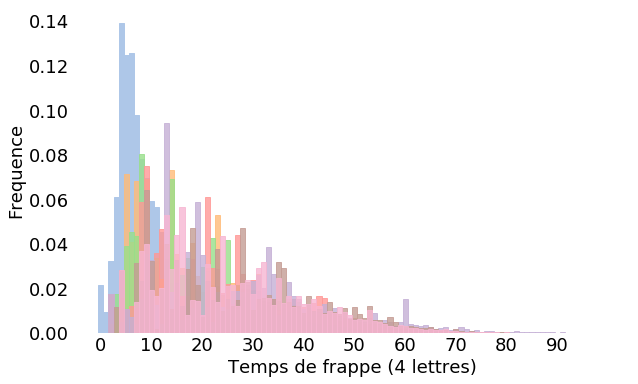
\includegraphics[scale=0.35]{distrib.png}
  \caption{Distribution du temps de frappe en fonction de la longueur des mots pour différentes méthodes. Bleu - recherche dichotomique, orange : épellation dichotomique, vert : alphabet EJASINT, rouge : 3, violet : 4, marron : 5, rose pâle : 6}
  \label{distrib}
\end{figure}
\end{center}

\begin{center}
\begin{figure}
  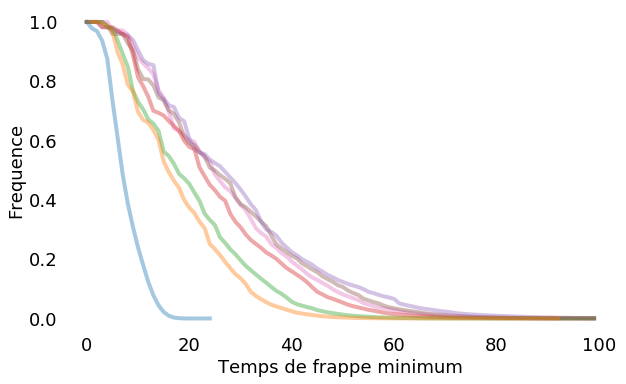
\includegraphics[scale=0.35]{frappe-mini.png}
  \caption{Proportion de mots ayant un temps de frappe donné. Bleu - recherche dichotomique, orange : épellation dichotomique, vert : alphabet EJASINT, rouge : 3, violet : 4, marron : 5, rose pâle : 6}
  \label{frappe-mini}
\end{figure}
\end{center}

\subsection{Moyenne et maximum}

Les distributions donnent beaucoup d'information sur les méthodes, mais les graphes sont difficilement lisibles. D'un point de vue pratique, on est principalement intéressés par le temps moyen nécessaire pour écrire un mot, et le temps maximal garanti.

La figure \ref{mean} montre que la recherche dichotomique a une longueur de frappe moyenne significativement plus faible que toutes les autres méthodes considérées, ce qui signifie que les mots sont en moyenne tapés trois à cinq plus vite. De plus, son écart-type plus faible donc il est peu probable d'avoir à écrire un mot fastidieux à écrire.

\begin{center}
\begin{figure}
  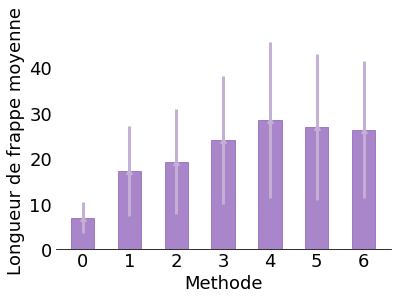
\includegraphics[scale=0.5]{mean.png}
  \caption{Longueur de frappe moyenne sur l'ensemble du dictionnaire (barre violettes), avec l'écart-type de la distribution (petites barres violettes claires). 0 - recherche dichotomique, 1 - épellation dichotomique, 2 - alphabet EJASINT, 3 à 6 - méthodes 3 à 6}
  \label{mean}
\end{figure}
\end{center}

Même si l'intervention de l'aidant permet souvent de trouver les mots sans épeler toutes les lettres, on peut s'intéresser au pire des cas, c'est-à-dire au mot du dictionnaire le plus long à trouver. On remarque sur la figure \ref{maxi} que la dichotomie sur le lexique offre une performance drastiquement meilleure que les autres méthodes, avec un facteur variant de quatre à sept.

\begin{center}
\begin{figure}
  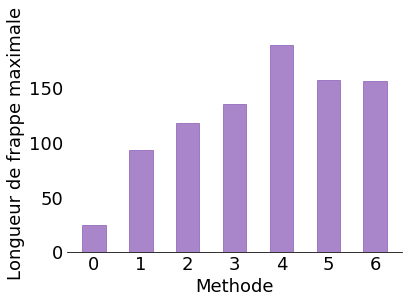
\includegraphics[scale=0.5]{frappe-maxi.png}
  \caption{Temps de frappe du mot le moins accessible. 0 - recherche dichotomique, 1 - épellation dichotomique, 2 - alphabet EJASINT, 3 à 6 - méthodes 3 à 6}
  \label{maxi}
\end{figure}
\end{center}

%------------------------------------------------

\section{Conclusion}

La méthode de recherche dichotomique utilisée par le projet Dicotomix est donc une méthode permettant, d'un point de vue théorique, d'écrire de façon significativement plus rapide que les méthodes actuelles. Cependant, elle nécessite un coût cognitif plus important, afin de répondre aux questions nécessaires à identifier un mot. 

%----------------------------------------------------------------------------------------
%	REFERENCE LIST
%----------------------------------------------------------------------------------------

% \begin{thebibliography}{99} % Bibliography - this is intentionally simple in this template

%\bibitem[Figueredo and Wolf, 2009]{Figueredo:2009dg}
%Figueredo, A.~J. and Wolf, P. S.~A. (2009).
%\newblock Assortative pairing and life history strategy - a cross-cultural
%  study.
%\newblock {\em Human Nature}, 20:317--330.
 
%\end{thebibliography}
%
%----------------------------------------------------------------------------------------

\end{document}
